\documentclass[
	article,
	11pt,
	oneside,
	a4paper,
	english,
	brazil,
	]{abntex2}

\usepackage{cmap}
\usepackage{lmodern}
\usepackage{adjustbox}
\usepackage[T1]{fontenc}
\usepackage[utf8]{inputenc}
\usepackage{indentfirst}
\usepackage{nomencl}
\usepackage{color}
\usepackage{graphicx}
\usepackage{listings}
\usepackage[colorinlistoftodos]{todonotes}
\graphicspath{ {./imagens/} }
\usepackage{lipsum}
\usepackage[brazilian,hyperpageref]{backref}
\usepackage[alf]{abntex2cite}
\renewcommand{\backrefpagesname}{Citado na(s) página(s):~}
\renewcommand{\backref}{}
\renewcommand*{\backrefalt}[4]{
	\ifcase #1 %
		Nenhuma citação no texto.%
	\or
		Citado na página #2.%
	\else
		Citado #1 vezes nas páginas #2.%
	\fi}
	
\definecolor{blue}{RGB}{41,5,195}

\makeatletter
\hypersetup{
		pdftitle={\@title}, 
		pdfauthor={\@author},
    	pdfsubject={Aps de Redes 1},
	    pdfcreator={LaTeX with abnTeX2},
		pdfkeywords={abnt}{latex}{abntex}{abntex2}{atigo científico}, 
		colorlinks=true,
    	linkcolor=blue,
    	citecolor=blue,
    	filecolor=magenta,
		urlcolor=blue,
		bookmarksdepth=4
}
\makeatother

\makeindex

\setlrmarginsandblock{2cm}{2cm}{*}
\setulmarginsandblock{2cm}{2cm}{*}
\checkandfixthelayout

\setlength{\parindent}{1.0cm}

\setlength{\parskip}{0.2cm}

\SingleSpacing

\begin{document}
\begin{titlepage}
    \begin{center}
        \vspace*{1cm}
            
        \Huge
        \textbf{Caminho de Dados de Ciclo Único e Controle MIPS}
            
        \vspace{0.5cm}
        \LARGE
            
        \vspace{1.5cm}
            
        \textbf{Ricardo Fedrigo, Caio Eduardo Theodoro}
            
        \vfill
            
        \vspace{0.8cm}
            
        \includegraphics[width=1.0\textwidth]{imagens/utfpr.png}
            
        \Large
        Coordenação do Curso de Bacharelado em Ciência da Computação - COCIC\\
        Universidade Tecnológica Federal do Paraná - UTFPR\\ 
        Campus Campo Mourão\\
        Campo Mourão, Paraná, Brasil\\            
    \end{center}
\end{titlepage}
\begin{abstract}
    Neste artigo, será documentado e detalhado os processos da implementação do subconjunto de instruções da arquitetura MIPS estudados na disciplina de Arquitetura e Desenvolvimento de computadores, e também tem como propósito, entender o Logisim e suas bibliotecas internas e externas.
\end{abstract}
\section{Funções basicas controlador:}
\subsection{Sinais de controle :}
Sinais de controle são um bloco com 9 entradas, que comandam os valores dos operadores do controlador, cada porta tem as seguintes propriedades:

        \begin{figure}[!htb]
        \centering
        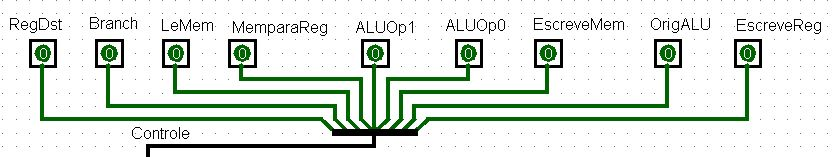
\includegraphics[scale=0.5]{imagens/SinaisDeControle.JPG}
        \caption{Sinais de controle}
        \label{fig:hostnetid}
        \end{figure}
        
\begin{itemize}
    \item \textbf{RegDst}: Determina qual o registrador de destino ( rt se 0, rd se 1).
    \item \textbf{EscreveReg}: Dá o sinal para escrever no registrador ( 0 para não, 1 para sim).
    \item \textbf{OrigALU}: Controla o multiplexador de seleção de entrada de dados. Ele faz a seleção de entrada de valor imediato ou de registrador.
    \item \textbf{Branch(ou OrigPC)} - Controla o multiplexador que atualiza o PC, caso 0, ele realiza PC+=4, caso 1, o PC segue para o desvio.
    \item \textbf{LeMem}: Controla a leitura da memoria, ( 1 para ler, 0 para não ler. note que somente a instrução lw tem permissão para leitura).
    \item \textbf{EscreveMem}: Controla a escrita da memoria, ( 1 para escrever, 0 para não escrever. note que somente a instrução sw tem permissão para escrita).   
    \item \textbf{MemparaReg}: Responsável pela seleção do multiplexador na saída da memória de dados. Ele Determina se a memoria de dados será salva em registrador.
\end{itemize}
\subsubsection{Decodificador :}

        \begin{figure}[!htb]
        \centering
        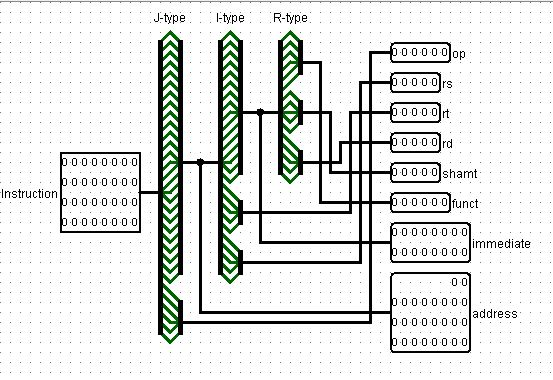
\includegraphics[scale=0.7]{imagens/Decodificador.JPG}
        \caption{Circuito do Decodificador}
        \label{fig:hostnetid}
        \end{figure}
O Decodificador é o bloco que recebe a memória da instrução, e a subdivide em três (3) formatos básicos, sendo cada uma responsavel por um tipo de operação ou conjunto de instrução, que são;

\begin{itemize}
    \item \textbf{I-Format} Referenciam operando da memória.
    \item \textbf{R-Format} Realizam operações em dados nos registradores.
     \item \textbf{J-Format} Incluem as instruções de desvio.
\end{itemize}

O tipo I é usado pelo lw, sw e beq na implementação, tipo R é usado para as operações aritmeticas add, sub, slt e or, já o tipo J, pelo jump. A Figura 3 mostra a divisão de bits de cada operação.

        \begin{figure}[!htb]
        \centering
        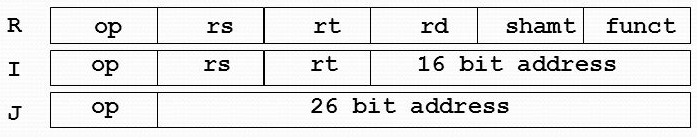
\includegraphics[scale=0.5]{imagens/FormatosInstrucao.png}
        \caption{Formatos de instrução}
        \label{fig:hostnetid}
        \end{figure}

Os canais do controlador partem para outras estruturas de controle do MIPS, como os registradores, o controle principal e o controle de ULA. 


\subsection{Controle da ULA:}

Para montar o controle da ULA, precisamos de duas entradas: ALUOp e Funct.
\begin{itemize}
  \item \textbf{ALUOp}: Recebemos dos sinais de controle ALUOp0 e ALUOp1, sendo 1 0 os ALUops das operações aritméticas. 
   \item \textbf{Funct}: Recebemos do decodificador, ela é responsável por sabermos qual operação(add, sub, or, slt e and). A Figura 4 mostra a relação da funct com as operações
\end{itemize}
        \begin{figure}[!htb]
        \centering
        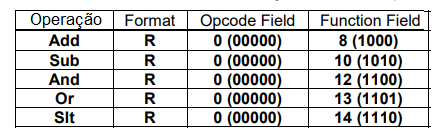
\includegraphics[scale=1.0]{imagens/operações.png}
        \caption{Operações}
        \label{fig:hostnetid}
        \end{figure}

\subsub{Controle da ULA Circuito:}
Montamos com isso por fim o ALUControl, tendo como saida a operação para a ULA. A Figura 5 mostra o circuito.

        \begin{figure}[!htb]
        \centering
        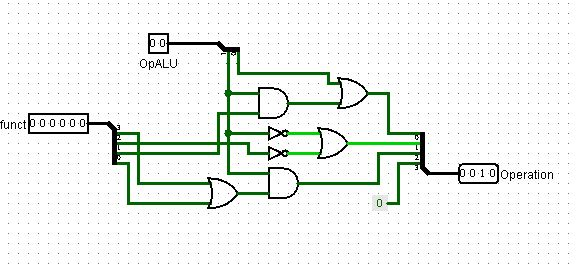
\includegraphics[scale=0.5]{imagens/ALUControl.JPG}
        \caption{Circuito ALUControl}
        \label{fig:hostnetid}
        \end{figure}

\subsection{Circuito}

Tendo feito a ALU, posicionar os multiplexadores e direcionado os caminhos do decodificador e dos sinais de controle, temos, por fim, o circuito manual do MIPS. A Figura 6 Mostra o circuito.


        \begin{figure}[!htb]
        \centering
        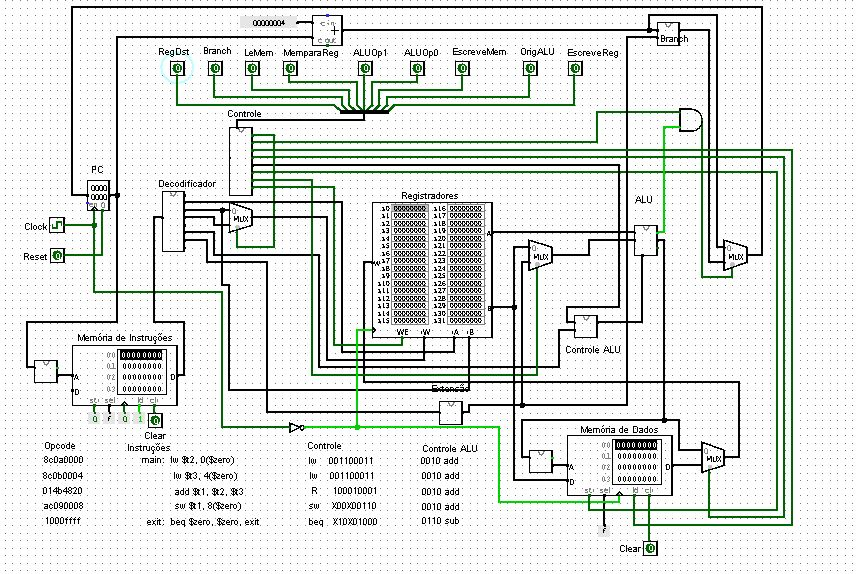
\includegraphics[scale=0.5]{imagens/circuito.JPG}
        \caption{Circuito Completo}
        \label{fig:hostnetid}
        \end{figure}

\subsection{Operações de teste}
Por fim, sera realizado a rotina do teste_1.asm. Com o código: 

\begin{lstlisting}
    .data
    .text
    .globl main
main:
    lw,$t2,0($zero)
    lw $t3.4($zero)
    add $t1,$t2,$t3
    sw, $t1,8($zero)
exit: beq $zero,$zero,exit
\end{lstlisting}


\subsubsection{lw $t2,0($zero)}
Primeiro temos lw $t2,0($zero), que tem a tabela de controle de sinais ilustrado na Tabela 1:

\begin{table}[h!]
  \centering
  \begin{adjustbox}{max width=\textwidth}
  \begin{tabular}{*{14}{|c}|}%%{|c|c|c|c|c|c|c|c|c|c|c|c|c|c|}
  \hline
  RegDst & EscreveReg &OrigALU & Branch & EscreveMem & LeMem & MemparaReg & OPcode\\
  \hline
  \hline
  $0$ & $1$ & $1$ & $0$ & $0$ & $1$ & $1$ &
  $00$ \\
  \hline
\end{tabular}
\end{adjustbox}
  \caption{Tabela controle para lw $t2,0($zero)}
  \label{tab:label_test}
\end{table}

Essa operação gera os estados no circuito ilustrados pelo Figura 8 : 

        \begin{figure}[!htb]
        \centering
        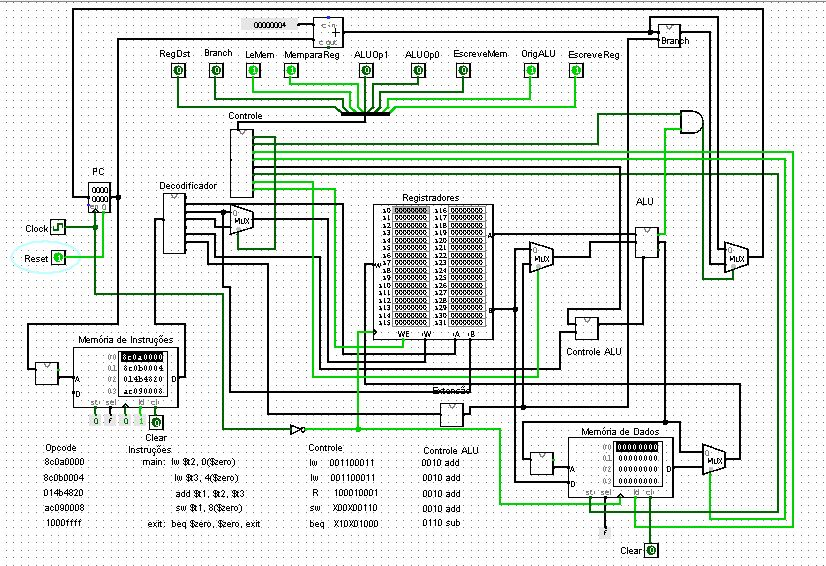
\includegraphics[scale=0.5]{imagens/teste_1.JPG}
        \caption{Controle MIPS para lw $t2,0($zero)}
        \label{fig:hostnetid}
        \end{figure}

\subsubsection{lw $t3,4($zero)}
Depois, temos lw $t3,4($zero), que tem a tabela de controle de sinais ilustrado na Tabela 2:

\begin{table}[h!]
  \centering
  \begin{adjustbox}{max width=\textwidth}
  \begin{tabular}{*{14}{|c}|}%%{|c|c|c|c|c|c|c|c|c|c|c|c|c|c|}
  \hline
  RegDst & EscreveReg &OrigALU & Branch & EscreveMem & LeMem & MemparaReg & OPcode\\
  \hline
  \hline
  $0$ & $1$ & $1$ & $0$ & $0$ & $1$ & $1$ &
  $00$ \\
  \hline
\end{tabular}
\end{adjustbox}
  \caption{Tabela controle para lw $t3,4($zero)}
  \label{tab:label_test}
\end{table}

Essa operação gera os estados no circuito ilustrados pelo Figura 9 : 

        \begin{figure}[!htb]
        \centering
        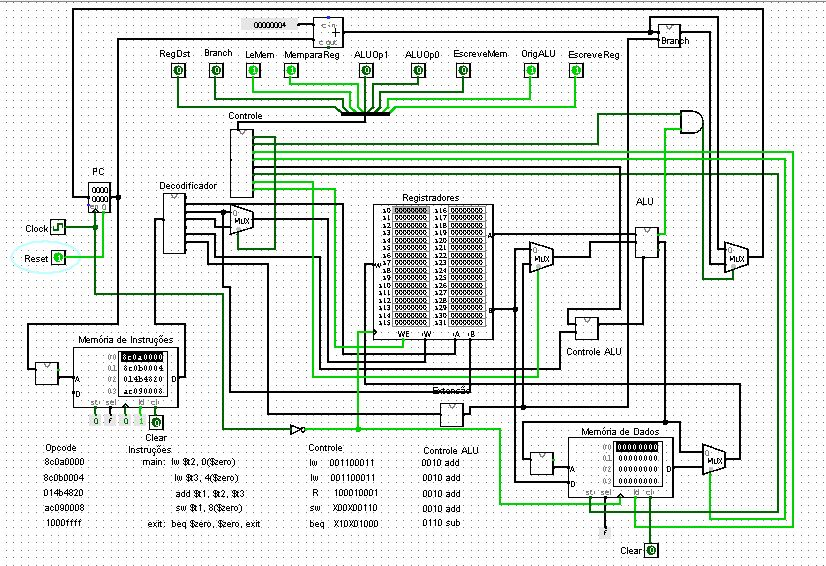
\includegraphics[scale=0.5]{imagens/teste_1.JPG}
        \caption{Controle MIPS para lw $t3,4($zero)}
        \label{fig:hostnetid}
        \end{figure}
        
\subsubsection{add t1,t2,t3}
Temos add t1, t2, t3, que tem a tabela de controle de sinais ilustrado na Tabela 3:

\begin{table}[h!]
  \centering
  \begin{adjustbox}{max width=\textwidth}
  \begin{tabular}{*{14}{|c}|}%%{|c|c|c|c|c|c|c|c|c|c|c|c|c|c|}
  \hline
  RegDst & EscreveReg &OrigALU & Branch & EscreveMem & LeMem & MemparaReg & OPcode\\
  \hline
  \hline
  $1$ & $1$ & $0$ & $0$ & $0$ & $0$ & $0$ &
  $10$ \\
  \hline
\end{tabular}
\end{adjustbox}
  \caption{Tabela controle para add $t1,$t2,$t3}
  \label{tab:label_test}
\end{table}

Essa operação gera os estados no circuito ilustrados pelo Figura 10 : 

        \begin{figure}[!htb]
        \centering
        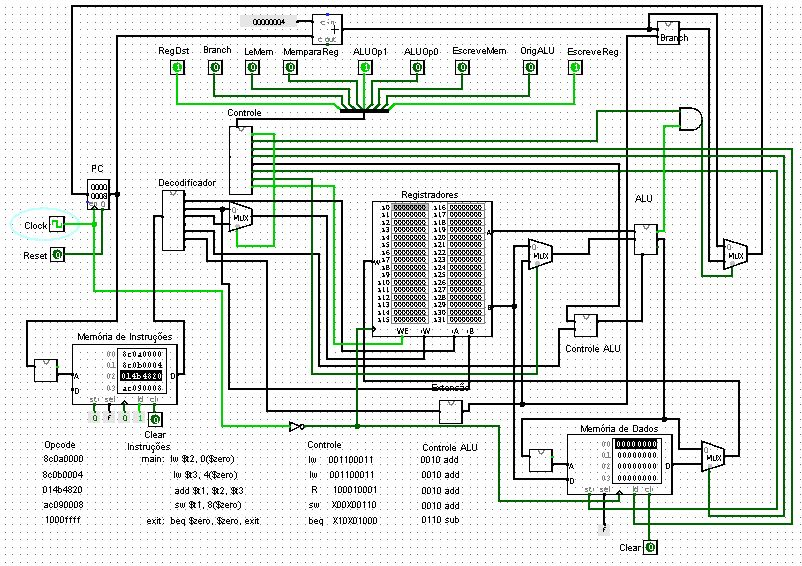
\includegraphics[scale=0.4]{imagens/teste_3.JPG}
        \caption{Controle MIPS para add $t1,$t2,$t3}
        \label{fig:hostnetid}
        \end{figure}

\subsubsection{sw $t1,8($zero)}
Temos sw $t1,8($zero), que tem a tabela de controle de sinais ilustrado na Tabela 4:

\begin{table}[h!]
  \centering
  \begin{adjustbox}{max width=\textwidth}
  \begin{tabular}{*{14}{|c}|}%%{|c|c|c|c|c|c|c|c|c|c|c|c|c|c|}
  \hline
  RegDst & EscreveReg &OrigALU & Branch & EscreveMem & LeMem & MemparaReg & OPcode\\
  \hline
  \hline
  $1$ & $1$ & $0$ & $0$ & $0$ & $0$ & $0$ &
  $00$ \\
  \hline
\end{tabular}
\end{adjustbox}
  \caption{Tabela controle para sw $t1,8($zero)}
  \label{tab:label_test}
\end{table}

Essa operação gera os estados no circuito ilustrados pelo Figura 11 : 

        \begin{figure}[!htb]
        \centering
        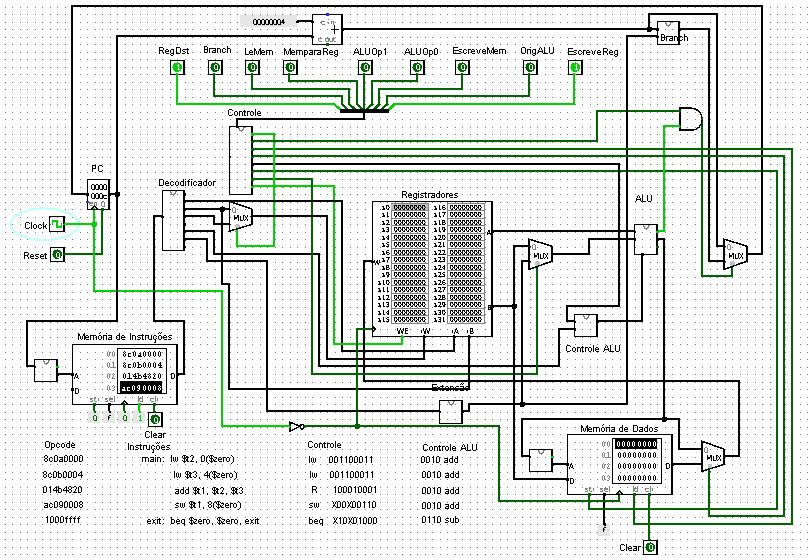
\includegraphics[scale=0.5]{imagens/teste_4.JPG}
        \caption{Controle MIPS para sw $t1,8($zero)}
        \label{fig:hostnetid}
        \end{figure}

\subsubsection{beq $zero,$zero,exit}
Temos beq $zero,$zero,exit, que tem a tabela de controle de sinais ilustrado na Tabela 5:

\begin{table}[h!]
  \centering
  \begin{adjustbox}{max width=\textwidth}
  \begin{tabular}{*{14}{|c}|}%%{|c|c|c|c|c|c|c|c|c|c|c|c|c|c|}
  \hline
  RegDst & EscreveReg &OrigALU & Branch & EscreveMem & LeMem & MemparaReg & OPcode\\
  \hline
  \hline
  $0$ & $0$ & $0$ & $1$ & $0$ & $0$ & $0$ &
  $01$ \\
  \hline
\end{tabular}
\end{adjustbox}
  \caption{Tabela controle para beq $zero,$zero,exit}
  \label{tab:label_test}
\end{table}

Essa operação gera os estados no circuito ilustrados pelo Figura 12 :
        \begin{figure}[!htb]
        \centering
        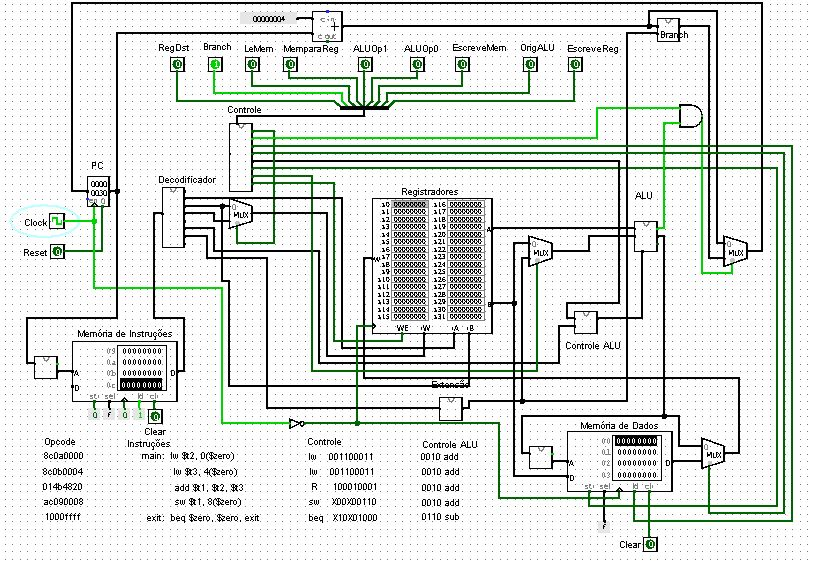
\includegraphics[scale=0.5]{imagens/teste_5.JPG}
        \caption{Controle MIPS para beq $zero,$zero,exit}
        \label{fig:hostnetid}
        \end{figure}
        
Após realizado  saída, o teste é finalizado.

\subsection{Conclusão}
Na discplina de Arquitetura e Redes de Computadores, torna-se fundamental o entendimento desses conceitos básicos de aplicação. A partir deles podemos, por fim, entender os componentes básicos da implementação de controle MIPS e Caminho de Dados de Ciclo Único.
\\
\\
\\
\begin{thebibliography}{2}

\bibitem{Patterson} 
Patterson, David A. - Hennessy, John L. 
\textit{Organização e Projeto de Computadores (5ª Edição)} . 
LTC Exatas Didático, 2017.

\bibitem{knuthwebsite} 
\textit{CA16 - MIPS control signals},
\\\texttt{https://www.youtube.com/watch?v=lqHKJyYCkXk}
\end{thebibliography}

\end{document}
O Decodificador é o bloco que recebe a memória da instrução, e a subdivide em três (3) formatos básicos, sendo cada uma responsavel por um tipo de operação ou conjunto de instrução, que são;


